\documentclass[titlepage,11pt,a4paper]{article}
\usepackage{tikz}
% \usepackage{bera}
\usepackage[T1]{fontenc}
\usetikzlibrary{shapes.geometric, arrows}
\usepackage{multirow}
\usepackage{graphicx}
\usepackage{caption}
\usepackage{subcaption}
\usepackage{floatrow}
\usepackage{amsmath}
\usepackage{float}
\floatstyle{plaintop}
\restylefloat{table}
\begin{document}

\title{\textbf{Software Systems Lab 4:\\TeX Lab}}
\author{Team Contour}
\date{12 August, 2017}
\maketitle

\newpage

% Flowchart
\begin{figure} 
\caption{Flowchart of a theist life}
\label{fig:f}
\tikzstyle{startstop} = [ellipse,minimum width=3cm,minimum height=1cm,text centered, draw=black, fill=white]
\tikzstyle{process} = [trapezium, trapezium left angle=70, trapezium right angle=110, minimum width=3cm, minimum height=1cm, text centered, draw=black, fill=white]
\tikzstyle{io} = [rectangle, minimum width=3cm, text width=2.5cm,minimum height=1cm, text centered, draw=black, fill=white]
\tikzstyle{decision} = [diamond, minimum width=3cm, minimum height=1cm, text centered,text width=1cm, draw=black, fill=white]
\tikzstyle{arrow} = [thick,->,>=stealth]

\begin{center}
\begin{tikzpicture}[node distance=1.5cm]
\node (start) [startstop] {Start Life};
\node (pray) [io, below of=start, yshift=-0.4cm] {Pray};
\node (work) [decision, below of=pray, yshift=-1cm] {Did it work?};
\node (praise) [io, below of=work, yshift=-1cm] {Praise the Lord};
\node (god) [io, below of=work, right of=praise, xshift =3cm, yshift=1.5cm] {God works in mysterious ways};
\node (die) [startstop, below of=praise,yshift=-0.3cm] {Die};

\draw [arrow] (start) -- (pray);
\draw [arrow] (pray) -- (work);
\draw [arrow] (work) -- (praise);
\draw [arrow] (work) -| (god);
\draw [arrow] (praise) -- (die);
\draw [arrow] (god) |- (die);
%\draw [arrow] (dec1) -- node[anchor=east] {yes} (pro2a);
\end{tikzpicture}
\end{center}
\end{figure}

% Paragraph
\paragraph{} Figure \ref{fig:f} above refers to a funny conundrum theists are believed to be living in by the atheists. This is just a joke I picked up from some forum, not taking sides, not even a bit. This is how scared social media has made us, We can not pick sides. Moving on\ .\ .\ .\ . You need to know how to cite papers in \LaTeX. For e.g. you are talking about research on Indowordnet \cite{indowordnet}, in that case such a citation must be used near a name. In case you need to quote the authors of a paper in a statement, instead of citing them against a topic or word or a line, you need to use a different kind of citation methodology.

\newpage

% % Table
\begin{table}[H] 
\caption{Table depicting the use of both multirow and multicolumn}
\label{table}
% For resizing the table to fit the page width
\resizebox{\linewidth}{!}{%
\begin{tabular}{c c|c|c|c|c|c|c|c|c|c|}
\cline{3-11}
& & \multicolumn{5}{c|}{\textbf{Basic Properties}} & \multicolumn{4}{c|}{\textbf{Readability}} \\ \cline{3-11}
& & \multicolumn{1}{|c|}{\textbf{WC}} & \textbf{SC} & \textbf{C-W} & \textbf{S-W} & \textbf{W-S} & \textbf{FK} & \textbf{GF} & \textbf{SMOG} & \textbf{LEX}\\ \cline{1-11}
\multicolumn{1}{|c|}{\multirow{2}{*}{\textit{Baseline}}} & Mean & 0.84 & 0.41 & \textbf{0.56} & \textbf{0.46} & \textbf{0.55} & \textbf{0.60} & 0.56 & 0.57 & 0.63\\ \cline{2-11}
\multicolumn{1}{|c|}{} & SD & 0.07 & 0.08 & 0.06 & 0.07 & 0.05 & 0.05 & 0.06 & 0.07 & 0.05\\ 
\hline \hline
 \multicolumn{1}{|c|}{\multirow{2}{*}{\textit{ScaComp$_{h}$}}} & Mean & 0.84 & 0.41 & \textbf{0.56} & \textbf{0.46} & \textbf{0.55} & \textbf{0.60} & 0.56 & 0.57 & 0.63\\ \cline{2-11}
\multicolumn{1}{|c|}{} & SD & 0.07 & 0.08 & 0.06 & 0.07 & 0.05 & 0.05 & 0.06 & 0.07 & 0.05\\ 
\hline \hline
\multicolumn{1}{|c|}{\multirow{2}{*}{\textit{ScaComp$_{l}$}}} & Mean & 0.84 & 0.41 & \textbf{0.56} & \textbf{0.46} & \textbf{0.55} & \textbf{0.60} & 0.56 & 0.57 & 0.63\\ \cline{2-11}
\multicolumn{1}{|c|}{} & SD & 0.07 & 0.08 & 0.06 & 0.07 & 0.05 & 0.05 & 0.06 & 0.07 & 0.05\\ 
\hline
\end{tabular}
}
\end{table}

\paragraph{} To combine rows a package must be imported with in your preamble, then you can use the XXXXXXX command in your document, I did it. The table below includes mathematical notations, which you can produce by embedding the experession in \$ \$ delimiters. For subscript, use underscore and for superscript, use carrot. 
\paragraph{} {\Large In table \ref{table} above, we try to demonstrate all the features required to be demonstrated in a table. We use multiple newline, we use a package to enable the use of multiple rows, and multiple columns in the table. Additionally, We have also drawn
lines from specific column to column. We also use box resizing with a width specifier for resizing the box within the limits of the document,  and avoid any overflow.}

\paragraph{} Now, we will import images side by side in the same document.

\newpage
\begin{figure}[H] \label{frow}
 \begin{floatrow} 
 \ffigbox{\caption{First figure}\label{fig1}}{\includegraphics[width=0.5\textwidth]{fig2}}
 \ffigbox{\caption{Second figure}\label{fig2}}{\includegraphics[width=0.5\textwidth]{fig3}}
 \end{floatrow}
 \end{figure}

\paragraph{} The images have been put in, and they are side by side in the same document on the same page. We have used the package floatrow and graphicx to import images on Page \pageref{frow}. The images are from an Android application I made for a project last semester. The table above are values from an experiment we are doing in our lab. I am adding an mathematical equation now just for the sake of it, because I think this is the only thing left to be demonstrated. 

\begin{equation} \label{eq1}
NLL=-\sum_{i=1}^{N}log(P(s_{i}))
\end{equation}
where $s_i$ is the length of the $i^{th}$ saccade.
\paragraph{} This text will refer to Equation \ref{eq1} above. In case you would like to see an alternative method to align the images, for instance images as subfigures, let me try to do it.
\newpage

% Alternate images

\begin{figure*}[t!]
    \centering
    \begin{subfigure}[t]{0.5\textwidth}
        \centering
        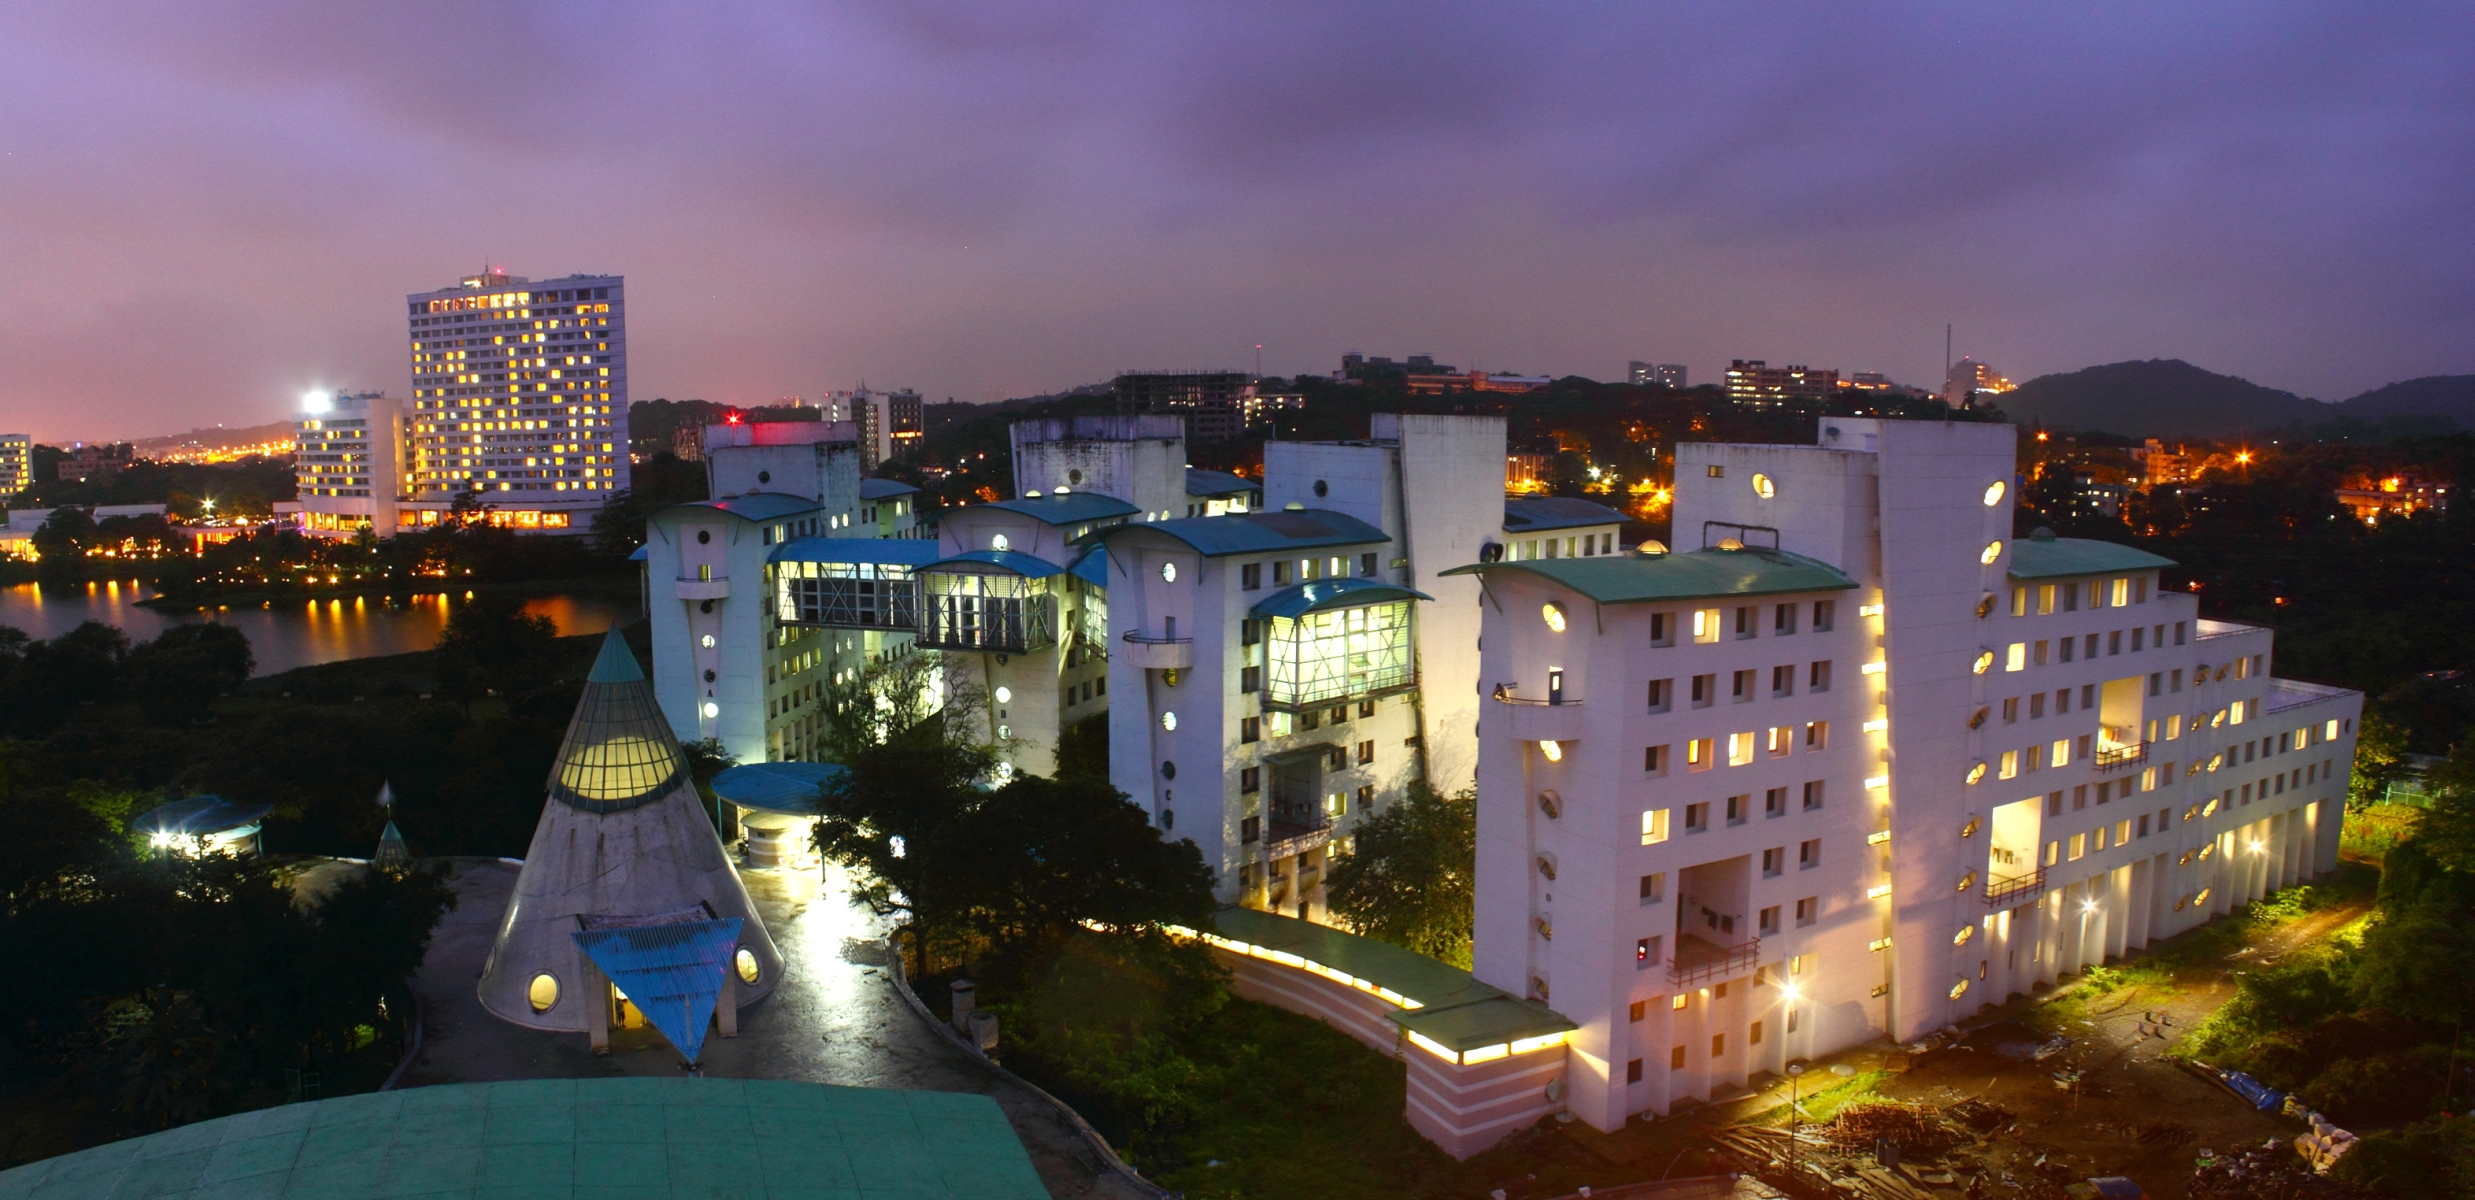
\includegraphics[height=1.2in,width=2in]{fig4_a}
        \caption{Caption 1}
    \end{subfigure}%
    ~ 
    \begin{subfigure}[t]{0.5\textwidth}
        \centering
        \includegraphics[height=1.2in,width=2in]{fig4_b}
        \caption{Caption 2}
    \end{subfigure}
    \caption{Caption for this figure with two images}
\end{figure*}

\paragraph{} This is another alternative to posting images in a \LaTeX\ Document, although you would still want me to put them in a table,  since `The Document' had them in a table. Let me try to do that.

\begin{table}[H]
\caption{Table with images, finally}
\begin{tabular}{c c}
\includegraphics[width=0.5\textwidth]{fig5} & \includegraphics[width=0.5\textwidth]{fig5} \\
\includegraphics[width=0.5\textwidth]{fig6} & \includegraphics[width=0.5\textwidth]{fig6}
\end{tabular}
\end{table}

\paragraph{} Now, that we have all the possible ways multiple images can be aligned in the table. We will conclude this document with the final
section. 

\newpage

% Conclusion
\section*{Conclusion} \label{end}
This document comprehensively demonstrated the capabilities of \LaTeX as a document typesetting / desktop publishing package. We have used various font size / family settings, we have used verbatim to display Latex code in a latex document, image settings, sections, subsections, references using labels, mathamatical equations, notations, use of ‘dia’ for creating a diagram / flowchart etc. I hope this suffices the need of learning basic \LaTeX. I hope you also notice that the last section i.e. Conclusion on Page \pageref{end} is unnumbered and displays the use of something.

% Bibliography
\begin{thebibliography}{9}
\bibitem{indowordnet}
Pushpak Bhattacharyya. Indowordnet. In \textit{The WordNet in Indian
Languages}, pages 1–18. Springer, 2017.
\end{thebibliography}

\end{document}